\documentclass{article}
\usepackage{tikz}
\newcommand{\hb}{\hbar}
\newcommand{\vv}{\vec}
\renewcommand{\vec}[1]{\mathbf{#1}}
\begin{document}
\begin{center}
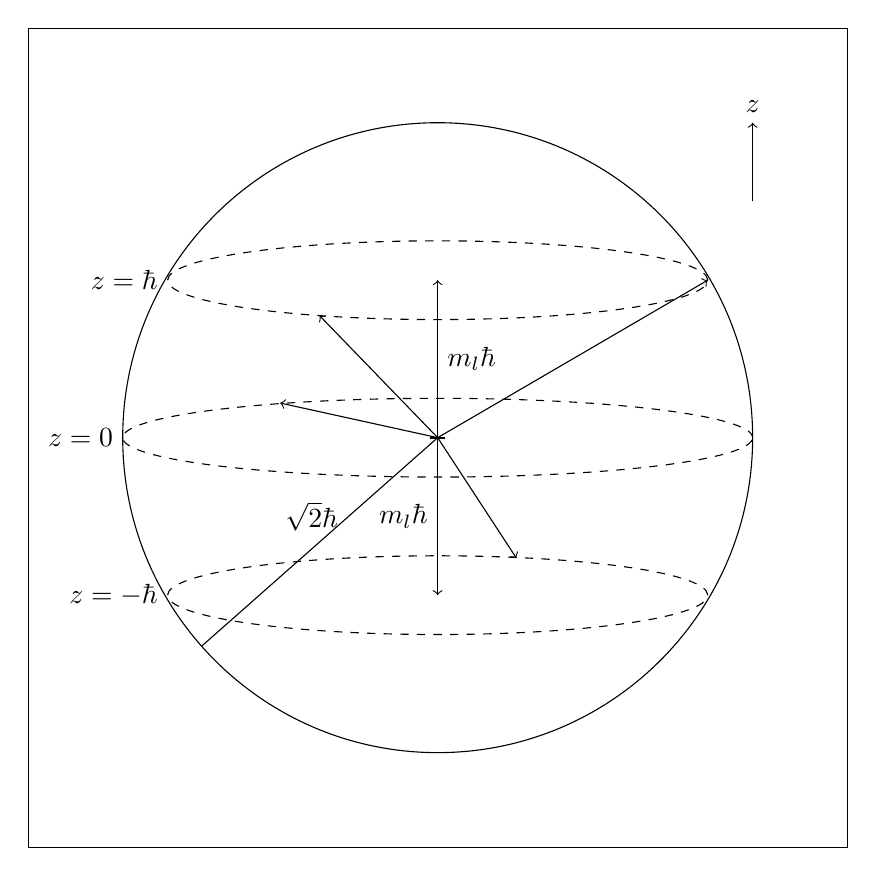
\begin{tikzpicture}
\draw (0,0) circle [radius=4];
\draw [dashed] (0,0) circle [x radius = 4, y radius = 0.5];
\draw [dashed] (0,2) circle [x radius = 3.43, y radius = 0.5];
\draw [dashed] (0,-2) circle [x radius = 3.43, y radius = 0.5];
\draw [|->] (0,0) -- (0,2);
\draw [|->] (0,0) -- (0,-2);
\draw [->] (0,0) -- (3.43,2);
\draw [->] (0,0) -- (-1.5,1.55);
\draw [->] (0,0) -- (-2, 0.44);
\draw [->] (0,0) -- (1,-1.53);
\draw (0,0) -- (-3,-2.65);
\draw [->] (4,3) -- (4,4);
\node [right] at (0,1) {\(m_l\hb\)};
\node [left] at (0,-1) {\(m_l\hb\)};
\node [left] at (-4,0) {\(z=0\)};
\node [left] at (-3.43, 2) {\(z=\hb\)};
\node [left] at (-3.43, -2) {\(z=-\hb\)};
\node at (-1.6,-1) {\(\sqrt 2\hb\)};
\node [above] at (4,4) {\(z\)};
\draw (5.2,5.2) -- (5.2,-5.2) -- (-5.2,-5.2) -- (-5.2,5.2) -- (5.2,5.2);
\end{tikzpicture}
\end{center}
\end{document}